The goal of this research is to be able to provide a system that makes use of an Arduino-based measuring device that can pass on data with a Bluetooth module to an Android phone that can be able to relay this data to a firebase database that can be accessed by another Android phone.

In order to be able to verify the temperature-humidity sensor being used, another device will serve as the basis for true data. Measurements coming from the TH-65, a digital temperature and humidity measuring device, will be established as ground truth.

The following graphs show the accuracy testing of the DHT-11 with the TH-65 as the basis for ground truth. The blue data represents the temperature measured by the DHT-11 while the orange represents data coming from the TH-65. Temperature, humidity, and discomfort index are to be considered in this set of data. From the results, it has been shown that in measuring temperature, the DHT-11 sensor shows 98.91\% accuracy and in humidity, the sensor is 89.66\% accurate in terms of measuring humidity and in discomfort index, the sensor is 97.79\% accurate. %The DHT-11 is shown to be 97.79\% accurate regarding the digital thermometer-hygrometer.

\begin{figure}[h]
\centering
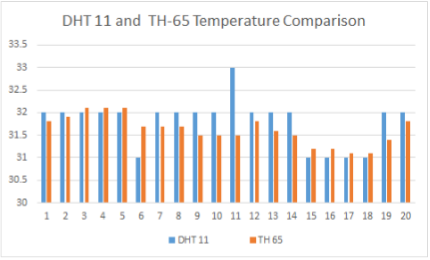
\includegraphics{Temperature}
\caption{Accuracy Testing of Temperature from DHT-11 sensor}
\end{figure}

\begin{figure}[h]
\centering
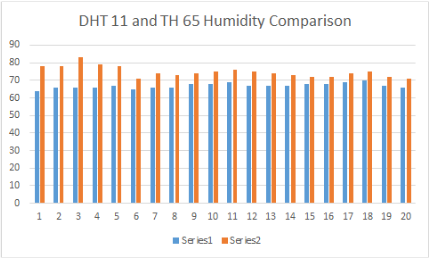
\includegraphics{Humidity}
\caption{Accuracy Testing of Humidity from DHT-11 sensor}
\end{figure}

\begin{figure}[h]
\centering
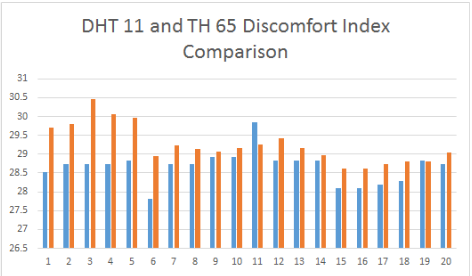
\includegraphics{DI}
\caption{Accuracy Testing of Discomfort Index from DHT-11 sensor}
\end{figure}

The Android application consists of viewing the database, checking the map, and updating the database. In updating the database, the data would simply come from the Arduino system transmitted via Bluetooth. The database is able to view the updated list of temperature, humidity, and discomfort index. The map shows the areas within DLSU that are color coded based on their discomfort indices. If the value shown is less than 21, the marker becomes blue. If it is between 21 to 24, the marker becomes cyan. If it is 24 to 27, the marker becomes azure. If it is between 27 to 29, the marker becomes orange. If it is between 29 to 32, the marker becomes rose. And if it is greater than 32, the marker becomes red.

\begin{figure}[h]
\centering
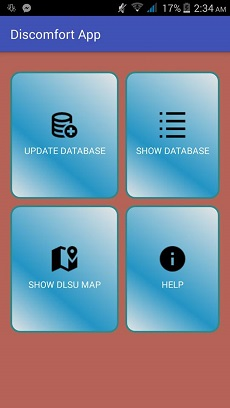
\includegraphics{Interface}
\caption{Interface for the Android Application}
\end{figure}

\begin{figure}[h]
\centering
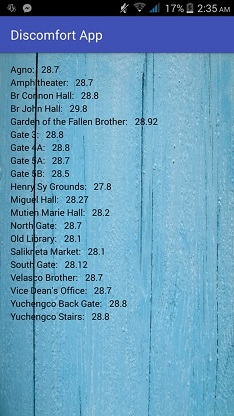
\includegraphics{Firebase}
\caption{The Updated List of Discomfort Indices Viewed from the Map}
\end{figure}

\begin{figure}[h]
\centering
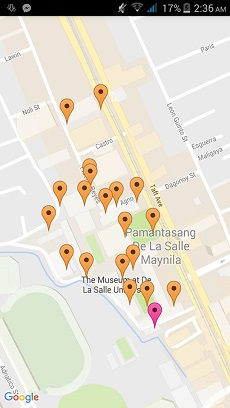
\includegraphics{Map}
\caption{Map of DLSU with Color Coded Markers Dictating the Discomfort Index}
\end{figure}

\begin{figure}[h]
\centering
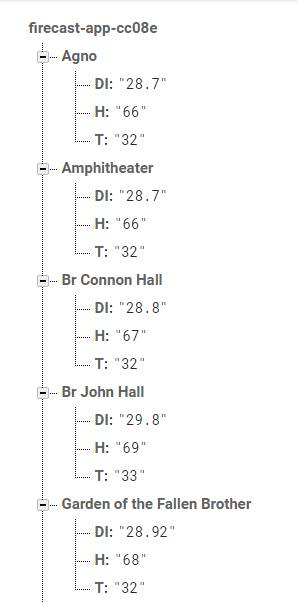
\includegraphics{Database}
\caption{A Part of the Firebase Database}
\end{figure}

\section{Summary}
The group has successfully developed an Arduino-based measuring device that takes note of temperature and humidity which can be transmitted via Bluetooth to an Android device and into an Android application. These data can be relayed onto the firebase database which will be accessible by all who has downloaded the application. The map inside is a handy feature that instantly tells the discomfort level of a certain area inside the university.